%% LyX 2.0.2 created this file.  For more info, see http://www.lyx.org/.
%% Do not edit unless you really know what you are doing.
\documentclass[12pt,a4paper,english,ngerman,intoc,bibliography=totoc,index=totoc,BCOR10mm,captions=tableheading,titlepage,fleqn]{scrbook}
\usepackage{lmodern}
\renewcommand{\sfdefault}{lmss}
\renewcommand{\ttdefault}{lmtt}
\usepackage[T1]{fontenc}
\usepackage[utf8]{inputenc}
\usepackage{fancyhdr}
\pagestyle{fancy}
\setcounter{secnumdepth}{3}
\setlength{\parskip}{\medskipamount}
\setlength{\parindent}{0pt}
\usepackage[ngerman]{babel}
\usepackage{amsmath}
\usepackage{amssymb}
\usepackage{graphicx}
\usepackage{nomencl}
\usepackage{booktabs}
\usepackage{listings}
\usepackage{tocbibind}
\usepackage{verbatim}
\usepackage{pdfpages}
\usepackage{color}
% the following is useful when we have the old nomencl.sty package
\providecommand{\printnomenclature}{\printglossary}
\providecommand{\makenomenclature}{\makeglossary}
\makenomenclature
\usepackage[unicode=true,
 bookmarks=true,bookmarksnumbered=true,bookmarksopen=true,bookmarksopenlevel=1,
 breaklinks=false,pdfborder={0 0 0},backref=false,colorlinks=false]
 {hyperref}
\hypersetup{pdftitle={Drehraten- und beschleunigungsbasierte Atemfrequenzmessung},
 pdfauthor={Gürkan Karacocuk},
 pdfsubject={Arbeit zur Erlangung des Masters der Technischen Fakultät der Albert-Ludwigs-Universität Freiburg im Breisgau},
 pdfkeywords={Masterarbeit},
 pdfpagelayout=OneColumn, pdfnewwindow=true, pdfstartview=XYZ, plainpages=false}

\makeatletter

%%%%%%%%%%%%%%%%%%%%%%%%%%%%%% LyX specific LaTeX commands.
\pdfpageheight\paperheight
\pdfpagewidth\paperwidth


\@ifundefined{date}{}{\date{}}
%%%%%%%%%%%%%%%%%%%%%%%%%%%%%% User specified LaTeX commands.
% Linkfläche für Querverweise vergrößern und automatisch benennen
\AtBeginDocument{\renewcommand{\ref}[1]{\mbox{\autoref{#1}}}}
\newlength{\abc}
\settowidth{\abc}{\space}
\AtBeginDocument{%
\addto\extrasngerman{
 \renewcommand{\equationautorefname}{\hspace{-\abc}}
 \renewcommand{\sectionautorefname}{Kap.\negthinspace}
 \renewcommand{\subsectionautorefname}{Kap.\negthinspace}
 \renewcommand{\subsubsectionautorefname}{Kap.\negthinspace}
 \renewcommand{\figureautorefname}{Abb.\negthinspace}
 \renewcommand{\tableautorefname}{Tab.\negthinspace}
 \renewcommand{\equationautorefname}{Gl.\negthinspace}
}
}

\newcommand{\pluseq}{\mathrel{+}=}
% für den Fall, dass jemand die Bezeichnung "Gleichung" haben will
%\renewcommand{\eqref}[1]{equation~(\negthinspace\autoref{#1})}

% Setzt den Link für Sprünge zu Gleitabbildungen
% auf den Anfang des Gelitobjekts und nicht aufs Ende
\usepackage[figure]{hypcap}

% Die Seiten des Inhaltsverzeichnisses werden römisch numeriert,
% ein PDF-Lesezeichen für das Inhaltsverzeichnis wird hinzugefügt
\let\myTOC\tableofcontents
\renewcommand\tableofcontents{%
  \frontmatter
  \pdfbookmark[1]{\contentsname}{}
  \myTOC
  %\mainmatter
 }

% make caption labels bold
\setkomafont{captionlabel}{\bfseries}
\setcapindent{1em}

% erlaubt LaTeX-Berechnungen
\usepackage{calc}

% fancy page header/footer settings
\renewcommand{\chaptermark}[1]{\markboth{#1}{#1}}
\renewcommand{\sectionmark}[1]{\markright{\thesection\ #1}}

% Vergrößert den Teil der Seite, in dem Gleitobjekte
% unten angeordnet werden dürfen
\renewcommand{\bottomfraction}{0.5}

% Vermeidet, dass Gleitobjekte vor ihrem Abschnitt gedruckt werden
\let\mySection\section\renewcommand{\section}{\suppressfloats[t]\mySection}

% deutscher Name für die Nomenklatur 
\renewcommand{\nomname}{Nomenklatur}

\makeatother


% Silbentrennungen
\hyphenation{Dreh-ra-ten-sen-so-ren}


\begin{document}


\subject{Masterarbeit}


\title{Drehraten- und beschleunigungsbasierte Atemfrequenzmessung}


\author{Gürkan Karacocuk}


\date{22. Dezember 2017}


%\publishers{\includegraphics{images/Uni_Logo-Grundversion_E1_A4_CMYK}\vspace{\baselineskip}\\
\publishers{\includegraphics{images/cover.png}\vspace{\baselineskip}\\
Albert-Ludwigs-Universität Freiburg im Breisgau\\
Technische Fakultät\\
Institut für Mikrosystemtechnik\vspace{-3cm}
}


\uppertitleback{Eingereichte Masterarbeit gemäß den Bestimmungen der Prüfungsordnung
der Albert-Ludwigs-Universität Freiburg für den Studiengang Master
of Science (M.\,Sc.) Embedded Systems Engineering vom 3.\,6.\,2014.}

\lowertitleback{\textbf{Bearbeitungszeitraum}\smallskip{}
\\
23.\,07.\,2017 -- 27.\,12.\,2017 \bigskip{}
\\
\textbf{Gutachter}\smallskip{}
\\
Prof.~Dr.~Leonhard~Reindl \bigskip{}
\\
Prof.~Dr.~YYY\bigskip{}
\\
\textbf{Betreuer}\smallskip{}
\\
Dr.-Ing. Fabian Höflinger}

\maketitle
\cleardoublepage{}

\pagestyle{empty}


\section*{Erklärung}

Hiermit erkläre ich, dass ich diese Abschlussarbeit selbständig verfasst
habe, keine anderen als die angegebenen Quellen/Hilfsmittel verwendet
habe und alle Stellen, die wörtlich oder sinngemäß aus veröffentlichten
Schriften entnommen wurden, als solche kenntlich gemacht habe. Darüber
hinaus erkläre ich, dass diese Abschlussarbeit nicht, auch nicht auszugsweise,
bereits für eine andere Prüfung angefertigt wurde.

\vspace{40mm}

Gürkan Karacocuk\\
Neuenburg, den 22. Dezember 2017

\cleardoublepage{}


\lhead{\rightmark}


\rhead[\leftmark]{}


\lfoot[\thepage]{}


\cfoot{}


\rfoot[]{\thepage}

\include{chapter/Zusammenfassung}

\selectlanguage{english}

\chapter*{Abstract}

%\addcontentsline{toc}{chapter}{Abstract} 

Abstract/Summary text\selectlanguage{ngerman}%



\tableofcontents{}


\listoffigures
\listoftables



\mainmatter

\cleardoublepage{}

\pagestyle{plain}

\cleardoublepage{}

\pagestyle{fancy}

\lhead[\chaptername~\thechapter]{\rightmark}


\lhead[\chaptername~\thechapter]{\rightmark}


\rhead[\leftmark]{}


\lfoot[\thepage]{}


\cfoot{}


\rfoot[]{\thepage}

\chapter{Einleitung}
Die Herzfrequenzmessung gehört seit jeher zur gängigsten Methode, um individuelle Belastungsbereiche eines Sportlers zu untersuchen. Dabei genügt heutzutage bereits eine handelsübliche Sportuhr. Somit kann die Herzfrequenz nicht-invasiv in Form eines tragbaren elektronischen Geräts (,,Wearable'') gemessen werden. Die Herzfrequenz stellt allerdings nur den kardiologischen Zustand dar und reicht deshalb nicht aus, um die vollständige Belastbarkeit eines Sportlers zu ermitteln. Hierfür muss unter anderem die Atemgasanalyse herangezogen werden. Bereits Mitte des 19. Jahrhunderts wurden nicht-invasive Atemmessungen, bei denen keine Geräte in den Körper eindringen, mittels Veränderungen der Körperoberfläche durchgeführt. Während erste Untersuchungen anhand der Silhouette von Probanden angestellt wurden, in denen die Brustkorbausdehnung seitlich betrachtet wurde, kann sie heutzutage durch verschiedene Methoden ermittelt werden. Die meisten Atemfrequenzuntersuchungen erfolgen allerdings stationär oder mithilfe einer Atemmaske, wie beispielsweise in der Ganzkörperplethysmographie oder Spirometrie und sind somit für viele Sportarten ungeeignet. Auch die Untersuchung von Säuglingen oder Tieren mit den genannten Methoden birgt viele Schwierigkeiten\cite{heyde}. In den letzten Jahren wurden einige Systeme entwickelt, die auf Basis von Inertialsensoren die Atemfrequenz bestimmen können. Dabei werden Sensoren rund um den Brustkorb angebracht, um dessen Ausdehnung zu erfassen. Anhand dieser Ansätze könnten in Zukunft Messmethoden entwickelt werden, die als Wearable während des Sports oder während der Schlafphase getragen werden können.

Die hier vorgelegte Abschlussarbeit beschreibt Anforderungen an ein System, das auf Intertialsensoren basiert. Dabei werden zuerst Untersuchungen an Probanden durchgeführt, um auf die bestmögliche Position auf dem Brustkorb für ein solches System schließen zu können. Zudem wird untersucht, wie groß ein Apparat dieser Art höchstens sein darf und welche Art von Bewegungen (Rotation oder Translation) dominieren. Des weiteren werden beide Inertialsensortypen (Beschleunigungs- und Drehratensensoren) gegenübergestellt und charakterisiert, inwiefern sie für eine Anwendung von Nutzen sein können. Abschließend wird ein Algorithmus für die Erfassung der Atemfrequenz im stationären und dynamischen Fall vorgestellt und anhand von Messungen validiert und diskutiert.


\lhead[\chaptername~\thechapter]{\rightmark}


\rhead[\leftmark]{}


\lfoot[\thepage]{}


\cfoot{}


\rfoot[]{\thepage}


\chapter{Theoretischer Hintergrund}
In diesem Kapitel werden die benötigten theoretischen Grundlagen für den Aufbau und das Verständnis der drehraten- und beschleunigungsbasierten Atemfrequenzmessung vorgestellt. Dabei werden wichtige Begriffe erläutert, die Funktionsweise von verwendeten Bauteilen erklärt und Methoden der Signalverarbeitung beschrieben.

\section{Atemmechanismus und -frequenz}
Der Atemmechanismus ist ein Vorgang, bei dem sich die Lunge ausdehnt, um Luft einzuatmen und kontrahiert, um Luft auszustoßen. Da die Lunge an sich kein Muskel ist, wird der Atemmechanismus von den Inspirationsmuskeln kontrolliert. Der wichtigste unter ihnen ist das Zwerchfell. Spannt es sich an, vergrößert sich der Brustkorb, was zu einem Unterdruck führt. Dieser Vorgang wird Inspiration genannt und in \ref{img:atemmechanik} (links) dargestellt. Um ausatmen zu können, muss sich das Zwerchfell entspannen, wodurch sich der Brustkorb verkleinert und die Luft durch den Überdruck nach draußen strömt. Der Vorgang der Expiration wird in \ref{img:atemmechanik} rechts illustriert\cite{anatomy-and-physiology}. 

\begin{figure}[h]
	\centering
	\includegraphics[width=0.55\textwidth]{images/atemmechanik.pdf}
	\caption[Atemmechanik]{Beim Einatmen vergrößert sich die Lunge (links) und beim Ausatmen verkleinert sie sich (rechts).}
	\label{img:atemmechanik}
\end{figure}

Wie in \ref{img:atemmechanik} zu erkennen, erfährt der Brustkorb eine deutliche Oberflächenveränderung während des Atemvorgangs. Neben der translatorischen Ausdehnung entsteht auch eine Drehung des vorderen Brustkorbs (Rotation).

\begin{table}[h!]
	\centering
	\caption{Atemfrequenzen von unterschiedlichen Altersgruppen}
	\label{tab:atemfrequenz}
	\begin{tabular}{lcc}
		\toprule
		Altersgruppe 	& \multicolumn{2}{c}{Atemfrequenz}\\
						& in Ruhe	& bei Belastung\\
		\midrule
		Säugling		& ca. 50 	& -\\
		Kindher			& ca. 25 	& ca. 70\\
		Erwachsene		& 12-16		& 40-60\\
		\bottomrule
	\end{tabular}
\end{table}

Die Atemfrequenz (\textit{engl. respiratory rate}) gibt an, wie oft in einer bestimmten Zeitspanne ein- und ausgeatmet wurde. Meistens wird die Zeitspanne in Minuten angegeben. Je nach Alter und gesundheitlichem Zustand variiert die Atemfrequenz eines Menschen. Die Atemfrequenzen für unterschiedliche Altergruppen werden in \ref{tab:atemfrequenz} aufgelistet\cite{juergen-weineck}. Die Frequenz erstreckt sich demnach von 12 bis 70 Atemzügen pro Minute bzw. 0,2 bis 1,2~Hz.

\section{Inertialsensoren}
Sensoren, die die Trägheit einer Masse nutzen, um auf sie einwirkende Kräfte zu messen, werden Inertialsensoren genannt (\textit{inert, lateinisch für ,,träge''}). Zu den Inertialsensoren werden Beschleunigungs- und Drehratensensoren gezählt. Der Anwendungsbereich erstreckt sich dabei von der Automobiltechnik über die Medizin bis hin zur Unterhaltungselektronik\cite{sensortechnik}.

	\subsection{Drehratensensoren}	
	MEMS-basierte Drehratensensoren (\textit{engl. gyroscope}) nutzen die Corioliskraft, um die Winkelgeschwindigkeit $^\circ/s$ um eine definierte Achse zu messen. Ein Drei-Achsen Drehratensensor ist so ausgelegt, dass er Rotationen im dreidimensionalen Raum erkennen kann. Rotationen um diese drei orthogonal zueinander stehenden Achsen werden Roll-, Nick- und Gier-Winkel (\textit{engl. roll-, pitch-, yaw-angle}) genannt und werden in \ref{img:rollpitchyaw} dargestellt. Bewegt sich ein Massepunkt $m$ mit der Relativgeschwindigkeit $v_{rel}$ in einem sich rotierenden Bezugssystem mit einer Drehgeschwindigkeit $\Omega$, so erfährt er eine Corioliskraft $F_c$. Dadurch entsteht eine Beschleunigung $a_c$ orthogonal zu $v_{rel}$ und der Rotationsachse von $\Omega$ und wird durch

	\begin{equation}
		\vec{a}_c = \frac{\vec{F}_c}{m} = 2\vec{v}_{rel} \times \vec{\Omega}
		\label{eqn:corioliskraft}
	\end{equation}
 
 	beschrieben. Kräfte, Beschleunigungen und Geschwindigkeiten werden in \ref{eqn:corioliskraft} dabei in Vektorform dargestellt, da sie im dreidimensionalen Raum auf den Massepunkt~$m$ einwirken\cite{sensortechnik}.
 
 	\begin{figure}[h]
 		\centering
 		\includegraphics[width=0.5\textwidth]{images/rollpitchyaw.pdf}
 		\caption[Roll-, Nick- und Gierachsen]{Schematische Darstellung eines Drei-Achsen-Drehratensensors. Dabei stehen alle Achsen orthogonal zueinander an einem gemeinsamen Mittelpunkt.	Rotationen um die drei Achsen werden als Roll-, Nick- und Gierwinkel bezeichnet.}
 		\label{img:rollpitchyaw}
 	\end{figure}
 
 	Das zugrunde liegende Prinzip eines MEMS-basierten Drehratensensors beruht auf dem Zweimassenschwinger, der in \ref{img:zweimassenschwinger} schematisch dargestellt wird. Dabei werden beide Massepunkte gegenphasig in Schwingung versetzt. Wenn das Bezugssystem mit der Drehgeschwindigkeit $\Omega$ rotiert wird, beginnen die Massepunkte zusätzlich orthogonal zur aufgespannten Ebene von Schwingungsrichtung und der Rotationsachse zu schwingen. Die daraus resultierende Coriolisbeschleunigung $a_c$ kann dann mithilfe eines angeschlossenen elektrischen Schaltkreises gemessen und die Drehgeschwindgkeit in $^\circ$/s ausgegeben werden\cite{sensortechnik}.
 	
 	\begin{figure}[h]
 		\centering
 		\includegraphics[width=0.57\textwidth]{images/zweimassenschwinger.pdf}
 		\caption[Schematische Darstellung eines Zweimassenschwingers]{Schematische Darstellung eines Zweimassenschwingers. Das rotierende Bezugssystem mit Rotationsgeschwindigkeit $\Omega$ regt die beiden Massepunkte so an, dass die Coriolisbeschleunigung $a_c$ entsteht.}
 		\label{img:zweimassenschwinger}
 	\end{figure}
 
 	Um aus der Winkelgeschwindigkeit den Winkel zu bestimmen, muss sie integriert werden. Da die erfassten Daten eines Drehratenratensensors diskret sind, werden sie in einem Mikrocontroller numerisch gemäß
 	
	\begin{equation}
	 	Winkel \pluseq Winkel + Drehrate/Abtastrate
	 	\label{eqn:gyrointegration}
 	\end{equation}
 	
 	integriert. Dabei taucht das übliche Problem des Gyroscope-Drifts auf, da in Ruhe eine systematische Abweichung ungleich Null vorliegt. Wird dieser Wert nach \ref{eqn:gyrointegration} integriert, entsteht eine wachsende Abweichung zum echten Winkel. Angenommen, ein Drehratensensor zeigt in Ruhe eine Abweichung von 1~$^\circ$/s an. So hätte der Winkel bereits nach einer Minute eine absolute Abweichung von 60~$^\circ$, ohne dass sich der Sensor je bewegt hat.
 
	\subsection{Beschleunigungssensoren}
	Ein Beschleunigungssensor (\textit{engl. accelerometer}) misst eine Kraft $F$, die durch eine Beschleunigung $a$ auf eine Masse $m$ einwirkt. Bei bekannter Masse kann die Beschleunigung durch das 2. Newtonsche Axiom
	
	\begin{equation}
		F = m \cdot a
		\label{eqn:newton}
	\end{equation}
	
	berechnet werden. Sie wird dabei in m/s$^2$ oder als Vielfaches der Erdbeschleunigung g = 9,81~m/s$^2$ angegeben. Für Beschleunigungssensoren ist die Erdbeschleunigung von besonderer Wichtigkeit, da sie zu jeder Zeit als Lot zur Erdmitte vorhanden ist. Dadurch kann ein Beschleunigungssensor ohne weiteres Werkzeug kalibriert werden\cite{sensortechnik}.
	
 	\begin{figure}[h]
		\centering
		\includegraphics[width=0.57\textwidth]{images/accelerometer2.pdf}
		\caption[Schematische Darstellung eines Beschleunigungssensors]{Schematische Darstellung eines uniaxialen MEMS-Beschleunigungssensors mit seismischer Masse und Gehäuse.}
		\label{img:accelerometer}
	\end{figure}

	In \ref{img:accelerometer} wird ein schematischer Aufbau eines MEMS-Beschleunigungssensors in uniaxialer Richtung dargestellt. Die seismische Masse ist dabei an beiden Seiten durch Federn an ein Gehäuse befestigt und kann sich in einer Achse (hier horizontal) bewegen. Bei Krafteinwirkung F$_a$ erfährt die seismische Masse eine Verschiebung, die anhand der festen Elektroden kapazitiv gemessen werden kann\cite{sensortechnik}.
	
 	\begin{figure}[h]
		\centering
		\includegraphics[width=0.4\textwidth]{images/koordinatensystem.pdf}
		\caption[Rotationen um eine Achse]{Rotation um den Winkel $\alpha$ eines Koordinatensystems entlang der X-Achse.}
		\label{img:koordinatensystem}
	\end{figure}
	
	Neben der Eigenschaft als Kalibrierungsgegenstand dient die Erdbeschleunigung auch dazu, Neigungen im Bezug zur Erdoberfläche zu bestimmen. Dies gilt insbesondere für Roll- und Nick-Winkel. Der Gier-Winkel kann nicht bestimmt werden, da diese Achse entlang der Erdbeschleunigung ausgerichtet ist. In \ref{img:koordinatensystem} wird beispielhaft die Koordinate eines gedrehten Einheitsvektors $\Vec{z}$ (blau) angezeigt. Der Vektor hat demnach die neuen Koordinaten $\Vec{z} = (0, \sin{\alpha}, \cos{\alpha})$. Die entstandene Rotation im dreidimensionalen Raum kann in Form einer Drehmatrix für alle drei Vektoren angegeben werden. Für Drehungen im dreidimensionalen Raum entstehen dadurch drei Drehmatrizen\cite{rui-zhang}
	
	\begin{equation}
		R_x(\phi) = 
		\begin{pmatrix}
			1 & 0 & 0\\
			0 & \cos{\phi} & \sin{\phi}\\
			0 & -\sin{\phi} & \cos{\phi}
		\end{pmatrix},
		\label{eqn:drehmatrix-x}
	\end{equation}
	
	\begin{equation}
		R_y(\theta) = 
		\begin{pmatrix}
			\cos{\theta} & 0 & -\sin{\theta}\\
			0 & 1 & 0\\
			\sin{\theta} & 0 & \cos{\theta}
		\end{pmatrix},
		\label{eqn:drehmatrix-y}
	\end{equation}
	
	\begin{equation}
		R_z(\psi) = 
		\begin{pmatrix}
			\cos{\psi} & \sin{\psi} & 0\\
			-\sin{\psi} & \cos{\psi} & 0\\
			0 & 0 & 1
		\end{pmatrix}.
		\label{eqn:drehmatrix-z}
	\end{equation}
	
	Die Drehmatrizen geben dabei die relative Winkeländerung im Bezug auf die einzelnen absoluten Achsen an. Für eine freie relative Bewegung um alle Achsen, müssen alle Matrizen zu einer Orientierungsmatrix multipliziert werden. Nun kommt es darauf an, wie die Koordinaten des zu drehenden Systems anfänglich definiert sind. Für Drehungen wie in \ref{img:rollpitchyaw} abgebildet, ist die Sequenz X-Y-Z geeignet. Die Orientierungsmatrix R$_\text{ges}$ für Rollwinkel $\theta$, Nickwinkel $\phi$ und Gierwinkel $\psi$ lautet demnach wie folgt:
		
	\begin{equation}
		R_\text{ges} = R_x \cdot R_y \cdot R_z = 
		\begin{pmatrix}
			\text{c}\theta~\text{c}\psi & \text{c}\theta~\text{s}\psi & -\text{s}\theta\\
			\text{c}\psi~\text{s}\theta~\text{s}\phi - \text{c}\phi~\text{s}\psi & \text{c}\phi~\text{c}\psi + \text{s}\theta~\text{s}\phi~\text{s}\psi & \text{c}\theta~\text{s}\phi\\
			\text{c}\phi~\text{c}\psi~\text{s}\theta + \text{s}\phi~\text{s}\psi & \text{c}\phi~\text{s}\theta~\text{s}\psi - \text{c}\psi~\text{s}\phi & \text{c}\theta~\text{c}\phi
		\end{pmatrix},
		\label{eqn:orientierungsmatrix}
	\end{equation}
	
	wobei $\text{s}$ und $\text{c}$ für $\sin$ und $\cos$ stehen\cite{rui-zhang}. Angenommen ein Beschleunigungssensor ist anfänglich so orientiert, dass die Erdbeschleunigung gänzlich auf die Z-Achse des Sensors in Form von $\Vec{g} = (0,0,1)$ wirkt und der Sensor keinen weiteren Beschleunigungen ausgesetzt ist. So ist die Ausgabe $G = (G_x, G_y, G_z)$ des Sensors definiert als
	
	\begin{equation}
		\frac{G}{|G|} = R_\text{ges} \cdot \Vec{g} \Rightarrow
		\frac{1}{\sqrt{G_x^2 + G_y^2 + G_z^2}}
		\begin{pmatrix}
		G_x\\
		G_y\\
		G_z
		\end{pmatrix} =
		\begin{pmatrix}
			-\sin{\theta}\\
			\cos{\theta}\sin{\phi}\\
			\cos{\theta}\cos{\phi}
		\end{pmatrix}.
	\end{equation}
	
	Der Winkel $\phi$ um die Roll-Achse kann dann mit
	
	\begin{equation}
		\phi = \tan^{-1}{\left(\frac{G_y}{G_z}\right)}
	\end{equation}
	
	berechnet werden, da die X-Komponente unabhängig von $\phi$ und somit trivial ist. Für die Berechnung von $\theta$ müssen die Y- und Z-Komponenten trigonometrisch nach
	
	\begin{equation*}
		\sqrt{\cos^2{\theta}\sin^2{\phi} + \cos^2{\theta}\cos^2{\phi}}
		= \cos{\theta} \cdot \underbrace{\sqrt{\sin^2{\phi} + \cos^2{\phi}}}_{1}
		= \cos{\theta}
	\end{equation*}
	\begin{equation*}
		\Rightarrow \cos{\theta} = \sqrt{G_y^2 + G_z^2}
	\end{equation*}
	
	zusammengeführt werden. Somit lässt sich der Nick-Winkel $\theta$ durch
	
	\begin{equation}
		\theta = \tan^{-1}{\left( - \frac{G_x}{\sqrt{G_y^2 + G_z^2}} \right)}
	\end{equation}
	
	berechnen\cite{mark-pedley}.
	
\section{Signalverarbeitung}
Ein Sensor muss meist eine sehr feine analoge Umgebung erfassen, die mit Störungen behaftet ist. Unter anderem entsteht Rauschen durch die Verstärkung des Signalpegels. Um ein verwertbares Signal für den Abnehmer zu bekommen, können einige Signalverarbeitungsschritte vollzogen werden, die im Folgenden erläutert werden.

	\subsection{Savitzky-Golay-Filter}
	
	\subsection{Bandpass-Filter}
	
	\subsection{Sensordatenfusion}

	\subsection{Komplementär-Filter}

	\subsection{Kalman-Filter}

	\subsection{Schnelle Fourier-Transformation}

\section{Fehlerrechnung}

\lhead[\chaptername~\thechapter]{\rightmark}


\rhead[\leftmark]{}


\lfoot[\thepage]{}


\cfoot{}


\rfoot[]{\thepage}

\chapter{Stand der Technik}
Dieses Kapitel befasst sich mit dem aktuellen Stand der Technik, wobei es um die Atemfrequenzanalyse mithilfe von Inertialsensoren geht. Es wird dabei zwischen drei Methoden unterschieden.

\section{Drehratenbasierte Atemfrequenzanalyse}
In seiner Bachelorarbeit stellt Dustin Kunzelmann ein Verfahren vor, mittels Drehratensensoren die Auslenkung des Brustkorbs zu erfassen (\textit{Gyroscope Based Breath Analysis - GBBA}). Dabei wird die Winkelgeschwindigkeit der Brustkorbauslenkung betrachtet. Um die relative Auslenkung des Brustkorbs von der absoluten Drehbewegung der Testperson unterscheiden zu können, wird am Rücken der Testperson ein weiterer Drehratensensor angebracht. Ein Mikrocontroller erfasst die Daten von den Sensoren und berechnet daraus die Atemfrequenz und leitet sie über ein integriertes Bluetoothmodul an ein Smartphone weiter. Die Methode hat gezeigt, dass mit Drehratensensoren unter statischen Bedingungen die besten Ergebnisse erzielt werden. Sobald die Testperson nicht in Ruhe ist, sondern periodische Bewegungen ausführt, wird die Atmung schlecht bis gar nicht detektiert\cite{gabba}.

\section{Beschleunigungsbasierte Atemfrequenzanalyse}
Die Atemanalyse mithilfe von Beschleunigungssensoren ist etwas gängiger und findet bereits in einigen Anwendungen statt. Im Folgenden werden zwei Ansätze vorgestellt.

	\subsection*{Brust- und Rückensensor}
	Ähnlich wie bei der drehratenbasierten Atemfrequenzanalyse werden Beschleunigungssensoren je auf der Brust und am Rücken angebracht (\textit{Acceleration Based Breath Analysis - ABBA}). Dabei reichen kleine Auslenkungen des Brustkorbs bereits aus, um die Änderung der Erdbeschleunigung zu detektieren. Da das Signalrauschen der beiden Sensoren sehr groß ist, werden verschiedene Schritte der Signalglättung respektive Filterung durchgeführt. Die Ergebnisse zeigen, dass das ABBA-System in der Lage ist die Atemfrequenz unter verschiedenen Umständen mit sehr geringen Abweichungen zu bestimmen. Hohe Genauigkeiten werden dabei in Ruhe und vor allem bei hoher sportlicher Aktivität erzielt\cite{abba}.

	\subsection*{Zwei parallele Brustsensoren}
	
	
	
\section{Drehraten- und beschleunigungsbasierte Atemfrequenzanalyse}

	\subsection*{Improvement of Dynamic Respiration Monitoring Through Sensor Fusion of Accelerometer and Gyro-sensor}



\lhead[\chaptername~\thechapter]{\rightmark}


\rhead[\leftmark]{}


\lfoot[\thepage]{}


\cfoot{}


\rfoot[]{\thepage}


\chapter{Systementwicklung}

\section{Anforderungen an das System}

	\subsection{N"otige Aufl"osung}
	
		\subsubsection*{Frequenz}
		
		\subsubsection*{Ausdehnung}

	\subsection{Gr"o"se}
	
	\subsection{Position am Brustkorb}
	
		\subsubsection*{Unter Belastungsbedingungen}
		Brustatmung
		
		\subsubsection*{In Ruhe}
		Bauchatmung
	
	\subsection{Rotations- und Translationsbewegungen}
	
\section{Verwendete ICs}

	\subsection{STM32F405RG}
	
	\subsection{MPU9250}
	
	\subsection{(Bluetooth-Modul)}
	
\section{Platinendesign}

\newpage

\section{Kalibrierung}

	\begin{figure}[h]
		\centering
		\includegraphics[width=1\textwidth]{images/kalibrierung_algo}
		\caption[Flow-Chart des Kalibrierungsalorithmus]{Der Kalibrierungsalorithmus berechnet den Offset der Drehratenratensensoren und die Erdbschleunigung der Beschleunigungssensoren in Ruhe. Nach Berechnung der Roll- und Nickwinkel wird der Gierwinkel mit der kleinsten Abweichung mittels sukzessiver Approximation in vier Schritten bestimmt. Zuletzt wird die Rotationsmatrix übergeben und die zukünftigen Messdaten mit ihr rotiert.}
		\label{img:kalibrierung-algo}
	\end{figure}

	\begin{figure}[h]
		\centering
		\includegraphics[width=1\textwidth]{images/Messergebnisse/calibration-sar-error}
		\caption[Abweichung der Voder- und Rückvektoren]{.}
		\label{img:kalibrierung-sar-error}
	\end{figure}

	\begin{figure}[h]
		\centering
		\includegraphics[width=1\textwidth]{images/kalibrierung_sar}
		\caption[Sukzessive Approximation]{Das Verfahren der sukzessiven Approximation wird verwendet, um den Gierwinkel zwischen den Vorder- und Hinterachsen zu bestimmen. Dabei wird bei jedem Schritt die Abweichung zueinander nach Rotation um den Gierwinkel berechnet und der Gierwinkel dann schrittweise approximiert.}
		\label{img:sar}
	\end{figure}


	\begin{table}[h!]
		\centering
		\caption{Arbeitsweise der Sukzessiven Approximation}
		\label{tab:sar}
		\begin{tabular}{ccccc}
			\toprule
			Schritt & \multicolumn{2}{c}{Abweichungen} & Addierter Winkel & Gesamtwinkel\\
			& Untereinander & Zum vorherigen & in $^\circ$& in $^\circ$\\
			\midrule
			1 & E$_{1,p}$ < E$_{1,n}$ 	& -	& +8  & 8 \\
			2 & E$_{2,p}$ < E$_{2,n}$ 	& E$_{2,p}$ < E$_{1,p}$	& +4 & 12\\
			3 & E$_{3,p}$ > E$_{3,n}$ 	& E$_{3,n}$ < E$_{2,p}$	& $-$2  & 10 \\
			4 & E$_{4,p}$ < E$_{4,n}$ 	& E$_{4,p}$ > E$_{3,n}$	& +0  & 10 \\
			5 & E$_{5,p}$ < E$_{5,n}$ 	& E$_{5,p}$ > E$_{3,n}$	& +0  & 10 \\
			6 & E$_{6,p}$ < E$_{6,n}$ 	& E$_{6,p}$ < E$_{3,n}$	& +0,25  & 10,25 \\
			\bottomrule
		\end{tabular}
	\end{table}


\lhead[\chaptername~\thechapter]{\rightmark}


\rhead[\leftmark]{}


\lfoot[\thepage]{}


\cfoot{}


\rfoot[]{\thepage}


\chapter{Messaufbau und -durchf"uhrung}
In diesem Kapitel werden alle Messaufbauten beschrieben und die durchgeführten Messungen erklärt. 

\section{Mechanischer Brustkorb}
In \ref{img:mech-bruskorb} wird der mechanische Brustkorb für die Untersuchung des Versatzes, die Änderung des Winkels über die Frequenz und Einflüsse der Zentripetalkraft auf die Sensoren dargestellt. Da die Schwingprüfanlage \textit{TIRAvib} nur translatorische Schwingungen erzeugen kann, wurde mithilfe eines Holzgestells ein menschlicher Brustkorb imitiert. Dabei werden zwei kurze Balken vertikal an ein Querbalken befestigt, wobei der vordere Balken über ein Scharnier an den Querbalken verbunden ist. Dadurch werden die translatorischen Bewegungen des \textit{TIRAvib} in Rotationsbewegungen umgewandelt. Mithilfe eines Frequenzgenerators kann die Frequenz und Amplitude der Rotationsbewegung eingestellt werden. Durch den Messaufbau können Atemfrequenzen und Brustkorbauslenkungen simuliert und für Charakterisierungs- und Kalibrierungszwecke eingesetzt werden.

\begin{figure}
	\centering
	\includegraphics[width=0.35\textwidth]{images/mechBrustkorb}
	\includegraphics[width=0.38\textwidth]{images/mechBrustkorb2.PNG}
	\caption[Mechanischer Brustkorb]{Mithilfe einer Schwingprüfanlage und einem Gestell aus Holz wird ein mechanischer Brustkorb für die Imitation der Atemfrequenz und Brustkorbauslenkung gebaut.}
	\label{img:mech-bruskorb}
\end{figure}

	\subsection{Versatz}
	Der Versatz gibt an, wie groß der Abstand zwischen den Messwerten der gleichen Zeiteinheit ist. Da die Daten vom Sensor zum Mikrocontroller über die serielle SPI-Schnittstelle übertragen wird und außerdem der Mikrocontroller die Daten sequentiell abfragt, muss der Versatz bekannt sein, um asynchrone Überlagerungen in der Signalverarbeitung zu vermeiden. \ref{img:versatz} illustriert beispielhaft, wie der Versatz zwischen zwei Signalen entsteht.
	
	\begin{figure}[h]
		\centering
		\includegraphics[width=0.7\textwidth]{images/versatz.PNG}
		\caption[Versatz zwischen zwei Signalen]{Aufgrund der sequentiellen Erfassung von Sensor und Mikrocontroller erfährt das blaue Signal eine Verschiebung um t$_\text{v}$.}
		\label{img:versatz}
	\end{figure}

	Für die Versatzmessung werden Brust- und Rückenplatine an dem vorderen Balken des mechanischen Brustkorbs befestigt, sodass sie die gleiche Schwinungung erhalten. und mit einer Frequenz von 100~Hz und einer Amplitude von 50~mV am Frequenzgenerator betrieben. Daraus resultiert eine hochfrequente Vibration, mit sehr spitzen Amplituden. Für die Versatzmessung wird die Abtastrate der Sensoren auf 1~kHz gesetzt, um möglichst viele Messpunkte zu erhalten.
	
	\subsection{Winkel pro Frequenz}
	
	\subsection{Zentripetalkr"afte und Erdbeschleunigung}
	
\newpage
	
\section{Kalibrierung}

	\subsection{Kalibrierung an einem Holzbalken}
	
	\begin{figure}[h]
		\centering
		\includegraphics[width=0.5\textwidth]{images/KalibrierungHolzgestell}
		\caption[Kalibrierung an einem Holzbalken]{...}
		\label{img:holzbalken}
	\end{figure}

	\subsection{Vergleich der Kalibrierung mit Referenzsystem}

\newpage

	\subsection{Kalibrierung an einer Testperson}
	
	\begin{figure}[h]
		\centering
		\includegraphics[width=0.5\textwidth]{images/Kalibrierung_Testperson}
		\caption[Kalibrierung an einer Testperson]{...}
		\label{img:testperson}
	\end{figure}


\lhead[\chaptername~\thechapter]{\rightmark}


\rhead[\leftmark]{}


\lfoot[\thepage]{}


\cfoot{}


\rfoot[]{\thepage}


\chapter{Ergebnisse und Diskussion}

\begin{figure}
	\centering
	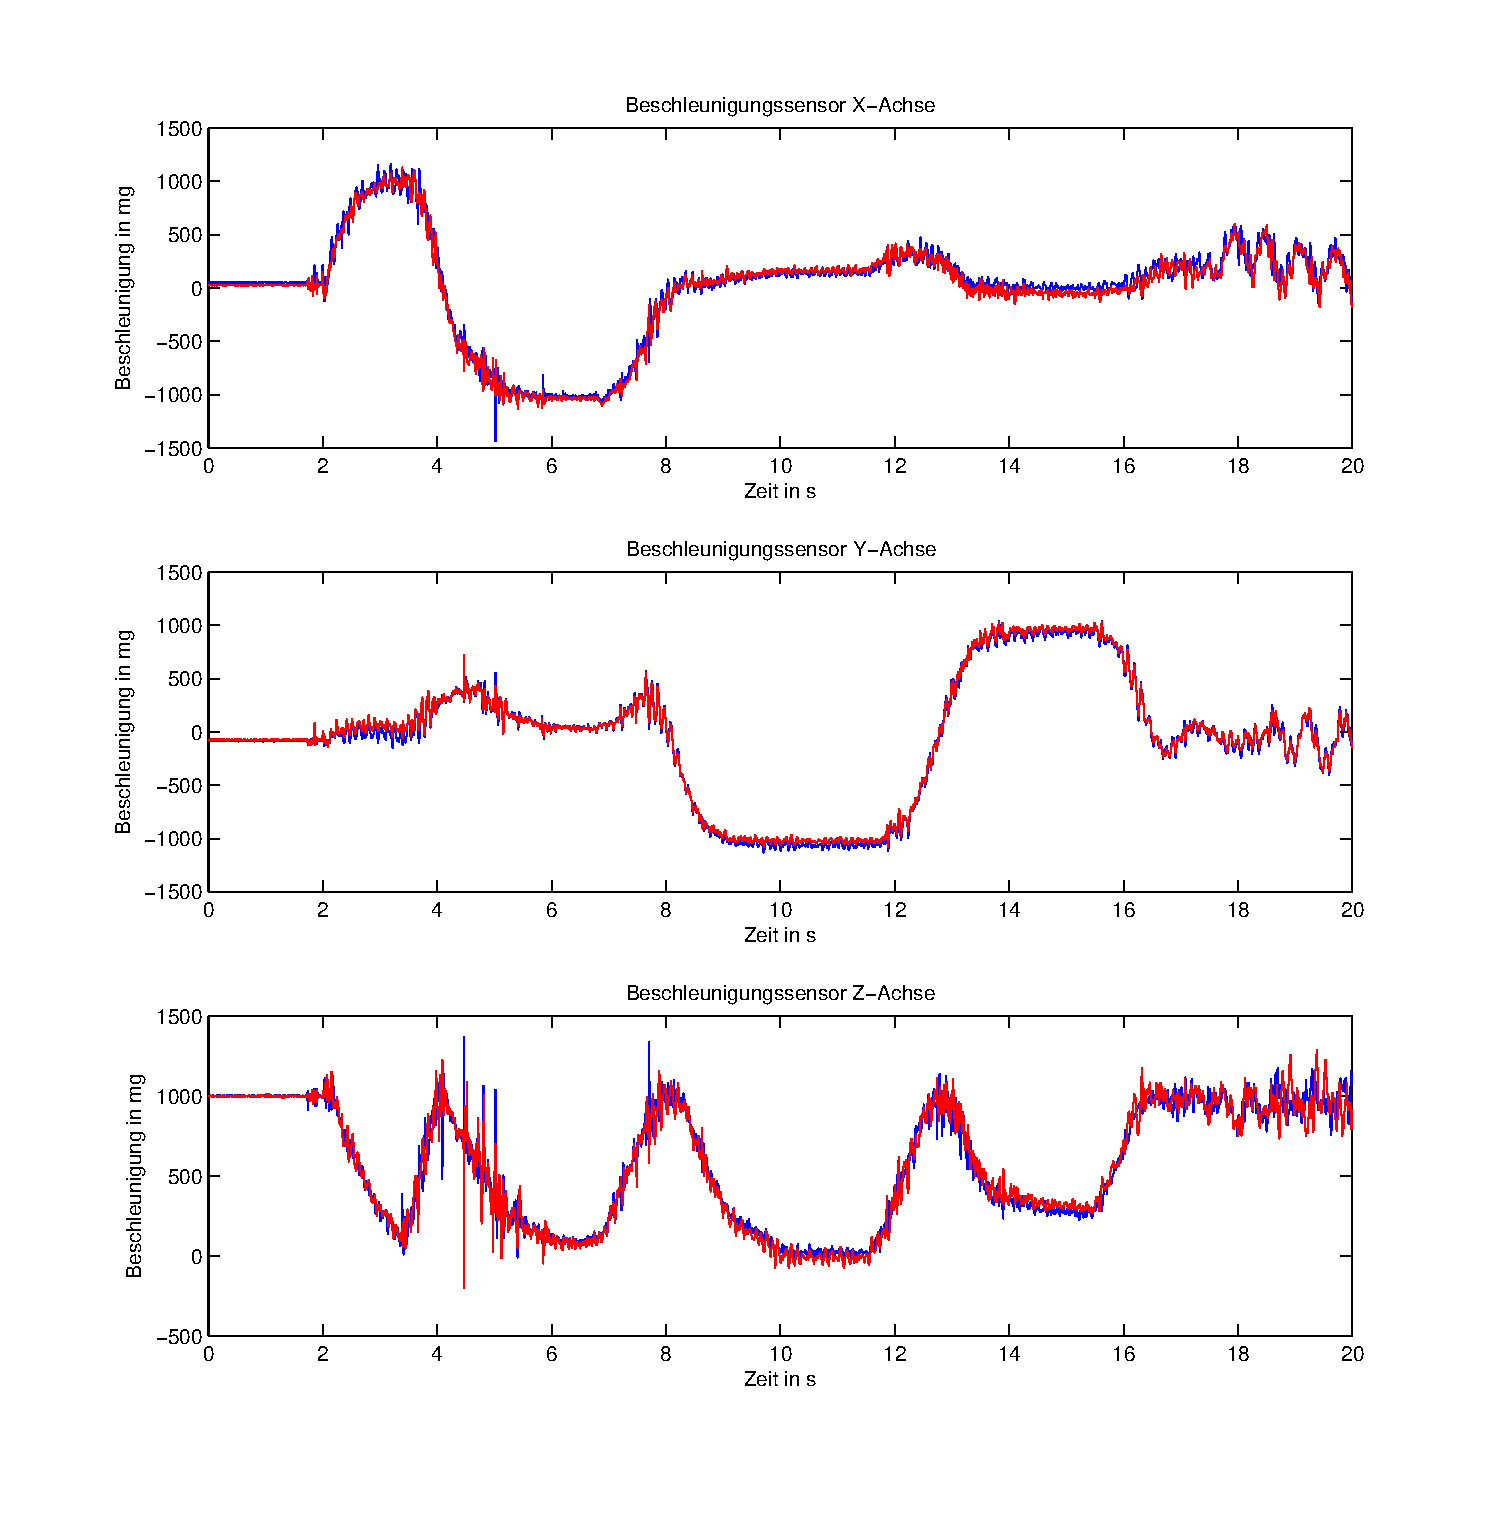
\includegraphics[width=1\textwidth]{images/Messergebnisse/calibration-wood-accel}
	\caption{Kalibrierung mit Holzgestell, Beschleunigungssensor.}
\end{figure}

\begin{figure}
	\centering
	\includegraphics[width=1\textwidth]{images/Messergebnisse/calibration-wood-gyro}
	\caption{Kalibrierung mit Holzgestell, Drehratensensor.}
\end{figure}

\begin{figure}
	\centering
	\includegraphics[width=1\textwidth]{images/Messergebnisse/calibration-wood-comparison}
	\caption{Kalibrierung Vergleich mit ABBA (Optimizer).}
\end{figure}

\begin{figure}
	\centering
	\includegraphics[width=1\textwidth]{images/Messergebnisse/calibration-faisal-move-accel}
	\caption{Kalibrierung mit Faisal, Beschleunigungssensor.}
\end{figure}

\begin{figure}
	\centering
	\includegraphics[width=1\textwidth]{images/Messergebnisse/calibration-faisal-move-gyro}
	\caption{Kalibrierung mit Faisal, Drehratensensor.}
\end{figure}

\begin{figure}
	\centering
	\includegraphics[width=1\textwidth]{images/Messergebnisse/calibration-faisal-chest-accel}
	\caption{Kalibrierung mit Faisal, Beschleunigungssensor, Bustatmung.}
\end{figure}

\begin{figure}
	\centering
	\includegraphics[width=1\textwidth]{images/Messergebnisse/calibration-faisal-chest-gyro}
	\caption{Kalibrierung mit Faisal, Drehratensensor, Brustatmung.}
\end{figure}

\begin{figure}
	\centering
	\includegraphics[width=1\textwidth]{images/Messergebnisse/calibration-faisal-tummy-accel}
	\caption{Kalibrierung mit Faisal, Beschleunigungssensor, Bauchatmung.}
\end{figure}

\begin{figure}
	\centering
	\includegraphics[width=1\textwidth]{images/Messergebnisse/calibration-faisal-tummy-gyro}
	\caption{Kalibrierung mit Faisal, Drehratensensor, Bauchatmung.}
\end{figure}




\lhead[\chaptername~\thechapter]{\rightmark}


\rhead[\leftmark]{}


\lfoot[\thepage]{}


\cfoot{}


\rfoot[]{\thepage}


\chapter{Fazit und Ausblick}

\cleardoublepage{}


\lhead[]{Danksagung}


\rhead[Danksagung]{}


\chapter*{Danksagung}

\addcontentsline{toc}{chapter}{Danksagung}

Bei Prof. Reindl m"ochte ich mich f"ur die M"oglichkeit bedanken, am Lehrstuhl f"ur Elektrische Mess- und Pr"ufverfahren an diesem Thema zu arbeiten und diese Arbeit zu verfassen.

Ein besonderer Dank gilt meinem Betreuer, Timo Kumberg f"ur seine Unterst"utzung, beim Entwerfen des Konzepts. Auch bei Herrn Robert Tannh"auser m"ochte ich mich f"ur seine Hilfsbereitschaft bedanken.

Nicht zuletzt geb"uhrt meinen Eltern Dank, ohne welche dieses ganze Unternehmen schon im Vorhinein niemals zustande gekommen w"are.

\appendix

\lhead[\chaptername~\thechapter]{\rightmark}


\rhead[\leftmark]{}


\lfoot[\thepage]{}


\cfoot{}


\rfoot[]{\thepage}

\chapter{Anhang}

\cleardoublepage{}


\lhead[]{\rightmark}


\rhead[\leftmark]{}

\bibliographystyle{biblio/unsrtdin}
\bibliography{biblio/Plasma}


\cleardoublepage{}


\lhead[]{Nomenklatur}


\rhead[Nomenklatur]{}

\printnomenclature[2.5cm]{}
\end{document}
